\documentclass[10pt]{standalone}
\usepackage[sc]{mathpazo}
\usepackage{commands}
\renewcommand{\phi}{\varphi}

\begin{document}
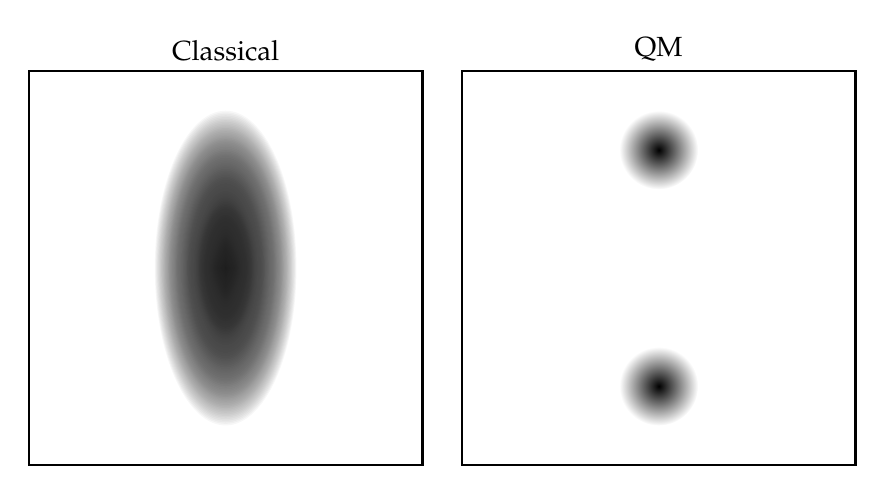
\begin{tikzpicture}[scale=1]
    \shade[even odd rule,inner color=black,outer color=white] (0,0) circle (0.5);
    \shade[even odd rule,inner color=black,outer color=white] (0,-3) circle (0.5);
    \draw[thick] (-2.5, -4) -- (-2.5, 1) -- (2.5, 1) -- (2.5, -4) -- cycle;
    \node[above] at (0, 1) {QM};

    \def\particles{(-5.5,-1.5) }
    \foreach \point in \particles{
    \foreach\i in {0,0.01,...,1.5} {
    \fill[opacity=\i*0.02,black] \point circle ({0.6-\i} and {1-2*\i});         
    }}
    \draw[thick] (-8, -4) -- (-8, 1) -- (-3, 1) -- (-3, -4) -- cycle;
    \node[above] at (-5.5, 1) {Classical};
\end{tikzpicture}
\end{document}